% ==============================================================
\chapter{Discussion and outlook}
% ==============================================================


\section{Decentralized MS/MS data evaluation infrastructure}



\begin{todo}
- decentralized system
- many researches, many computers for data evaluation
- low impact of failing single computers on overall performance 
- functional data evaluation setup can be restored in a straightforward way
- automatic software downloading
- also beneficial in education
- two-level design (CLI and GUI) allows for usage in situations which too 
  complex to be feasible for handling in the GUI
- rapid deployment of novel functionality
- support for multiple scripting languages

outlook:
- more functionality
- in particular, free de novo tool
- remote execution (but local creation)
- refinement of the workflow interaction metaphors (batches should be defined
  per arrow, not per input file box)
\end{todo}

However, TPP requires the installation of an Apache web server for the purpose
of providing a web browser-based graphical user interface (GUI).
While the graphical user interaction is helpful for users, the required Apache 
web server presents a non-negligible security risk because it potentially renders 
the user's computer accessible and exploitable from the Internet when it can be 
expected that most users won't be aware of this issue and will therefore not 
be able to regularly apply security patches. 
This issue is especially precarious on Windows and Mac OS X which do not 
natively provide centralized, automatic software updating.

\paragraph{High-throughput data processing.}

\paragraph{Rapid deployment of novel functionality.}

\section{Automated quantitation of metabolically labeled samples}

One of the studies presented in this thesis provides a comprehensive list of 
experimentally deduced chloroplast proteins for \cre~for the first time.
In addition, the anaerobic response of the chloroplast proteome of the green 
alga is characterized. 
Among other results, the induction of hydrogenase, a protein involved in 
hydrogen production, is confirmed \citep{Terashima2010}.

\section{Advancement of the Genomic Peptide Finder }

In 2007, GPF was redesigned and implemented from scratch in the scope of this
thesis to add a variety of features \citep{Specht2011_GPF}:

\begin{itemize}
\item intron splits may occur within a single coding nucleotide triplet
\item splice donor/acceptor site consensus sequences may be specified to
reduce the number of spurious spliced peptide alignments
\item increased search speed by employing an indexing strategy while locating
the occurences of sequence tags in the genomic DNA sequence
\end{itemize}

In addition, a method for the automated validation of GPF candidate peptides,
employing standard database search programs such as OMSSA was established.
This allows for statistically robust identification of GPF-deduced peptides
alongside gene model peptides.
Furthermore, an annotation pipeline was established in which resulting GPF
peptides are passed to AUGUSTUS, which performs an {\em ab initio} gene 
model prediction supplemented by various extrinsic hint sources including
GPF peptides.
It is therefore a major contribution of this thesis that an automated
proteogenomic annotation of the \cre~genome in which MS/MS data generated
for various unrelated purposes can be re-used for the generation of
extrinsic AUGUSTUS hints has become possible.

\paragraph{GPF-supported proteogenomic genome annotation.}

\begin{SCtopfig}
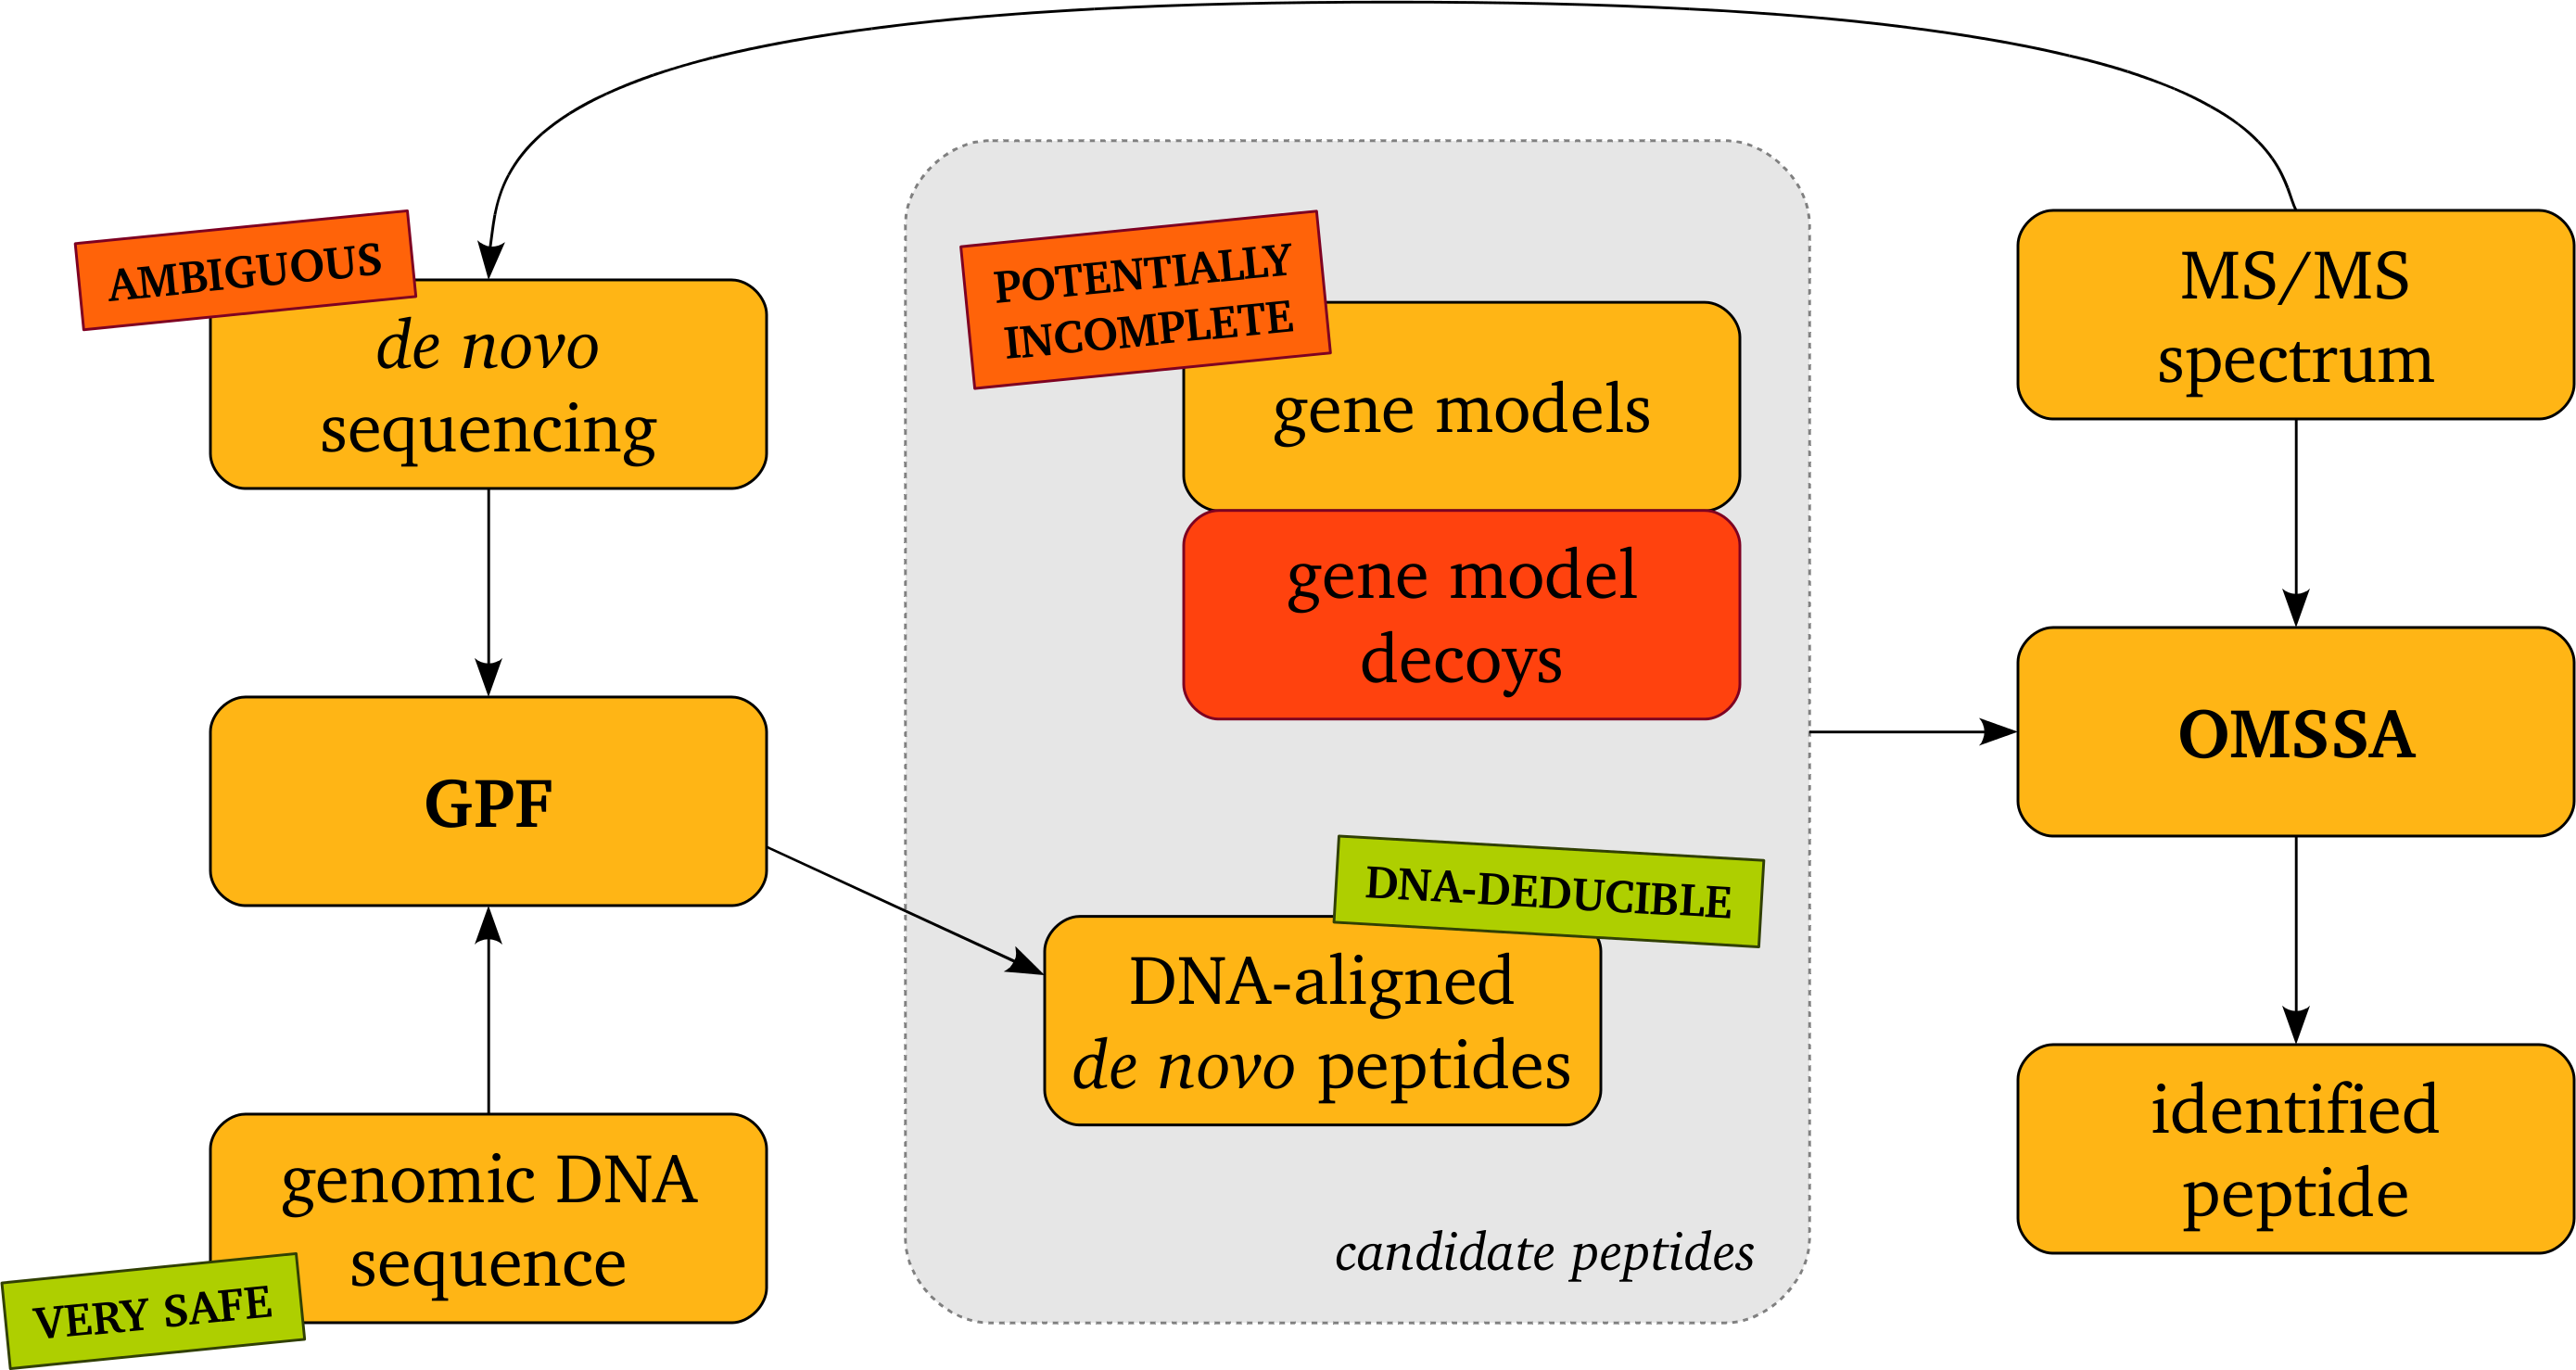
\includegraphics[width=0.7\textwidth]{figures/gpf-omssa.jpg}
\caption{
{\bf Validation of GPF candidate peptides via a target/decoy approach
    using previously established gene models.} 
    Statistical significance of identified GPF candidate peptides is 
    assessed using existing gene models which may be incomplete but
    can be expected to contain a high amount of correct sequences.
}
\label{fig:gpf-omssa}
\end{SCtopfig}

The GPF annotation pipeline presented in this thesis follows a similar strategy
(\cite{Specht2011_GPF}, see p.~\pageref{section:gpf} and \pageref{paper:gpf}).
However, the GPF approach is less biased in comparison to the exon splice graph
approach because it does not require exon/intron prediction as a first step.
GPF candidate peptides are solely generated from MS/MS {\em de novo} sequencing
and subsequent mapping of the resulting peptides to the genome, using 
a user-defined maximum intron length and a set of possible splice donor/acceptor 
site consensus sequences.
This means that intron prediction is carried out on a per-peptide basis, and
all peptides are treated independently.
The actual validation of extrinsic hints and splice site detection is
carried out by AUGUSTUS in the final annotation step.
Moreover, the approach is highly flexible because no specialized database
search program is required because candidate peptides are inferred by GPF
and then passed down the evaluation pipeline alongside a protein database
(see Fig.~\ref{fig:gpf-omssa}).
Although the protein database is used to estimate the FDR of peptide 
identifications, the final GPF-deduced peptides which are exported as
peptide hints do not originate from this database, although in the case
of \cre, a big portion of these protein database peptides could be 
independently confirmed via GPF \citep{Specht2011_GPF}.


\paragraph{Proteogenomic genome annotation.}

\paragraph{Identification of novel targets for reverse-genetics approaches.}
